\section{Experimentación}

Quisimos estudiar el comportamiento de nuestros algoritmos con instancias reales. Para ello corrimos el programa con instancias generadas aleatoriamente, siguiendo una distribución uniforme. Generamos casos de test con distintos valores de N (cantidad de elementos) para cada algoritmo. Como nuestras instancias fueron generadas aleatoriamente, corrimos numerosas veces los algoritmos y tomamos el promedio de sus tiempos, evitando así caer en casos extremos.
Una vez que obtuvimos los datos, comparamos nuestros resultados con las cotas asintóticas calculadas previamente .


\subsection{Experimentación sobre el algoritmo de Fuerza Bruta}
Para el algoritmo de Fuerza Bruta, notamos que no importa el valor de la instancia pues siempre calculamos todo el espacio de soluciones, lo que si importa es su tamaño. Como vimos en la sección anterior, tenemos una cota teórica de O($n*2^{n}$). Para ver que tan bien se ajusta nuestro algoritmo a ésta cota, experimentamos generando instancias aleatorias variando N entre 0 y 30. Veamos los resultados:

\begin{figure}[H]
   \begin{minipage}{0.5\textwidth}
     \centering
     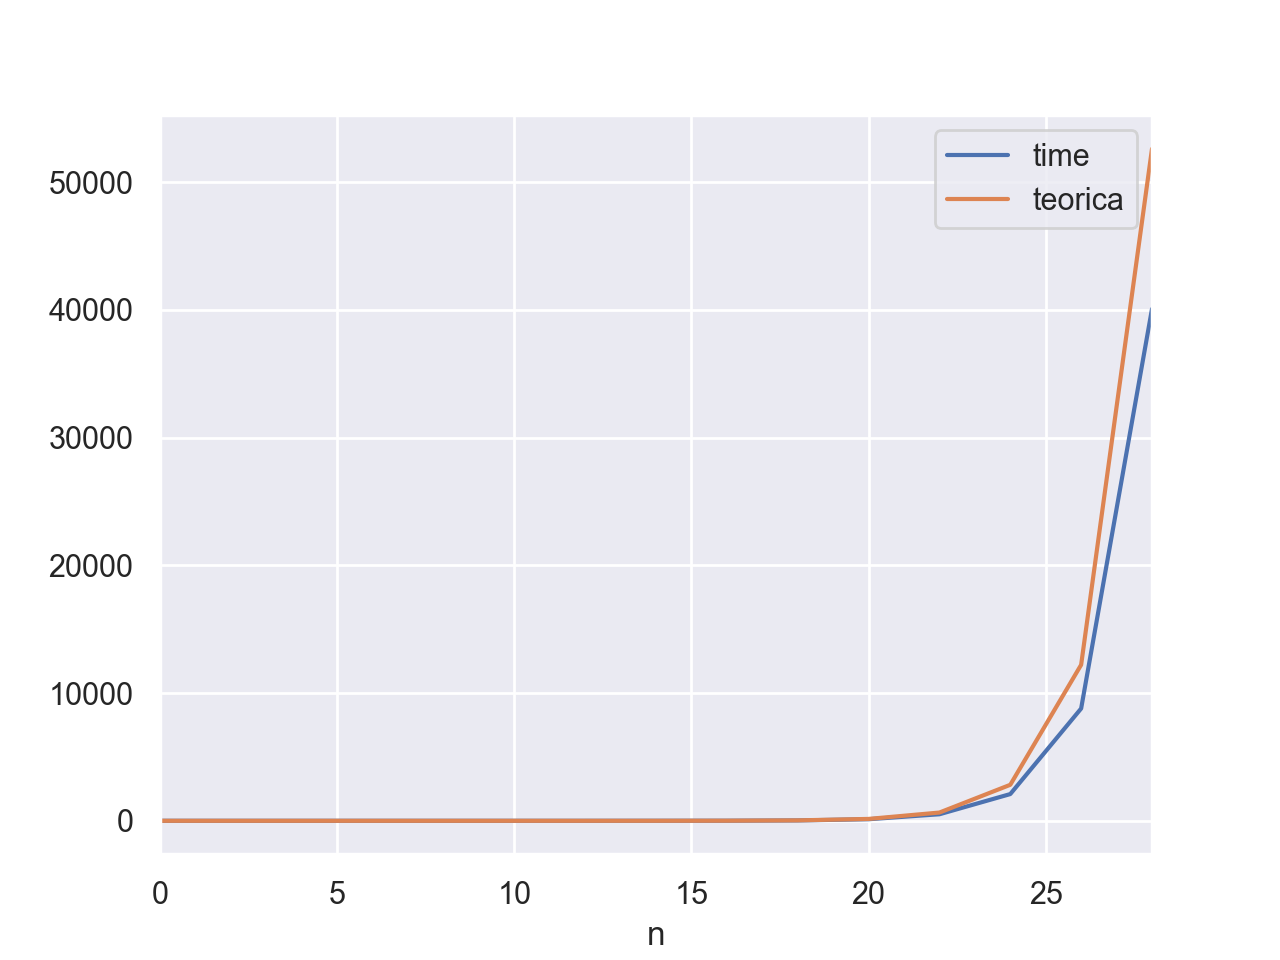
\includegraphics[width=1\linewidth]{img/fb_1}
     \caption{Comparación del gráfico de los resultados contra la cota teórica}
   \end{minipage}\hfill
   \begin{minipage}{0.5\textwidth}
     \centering
     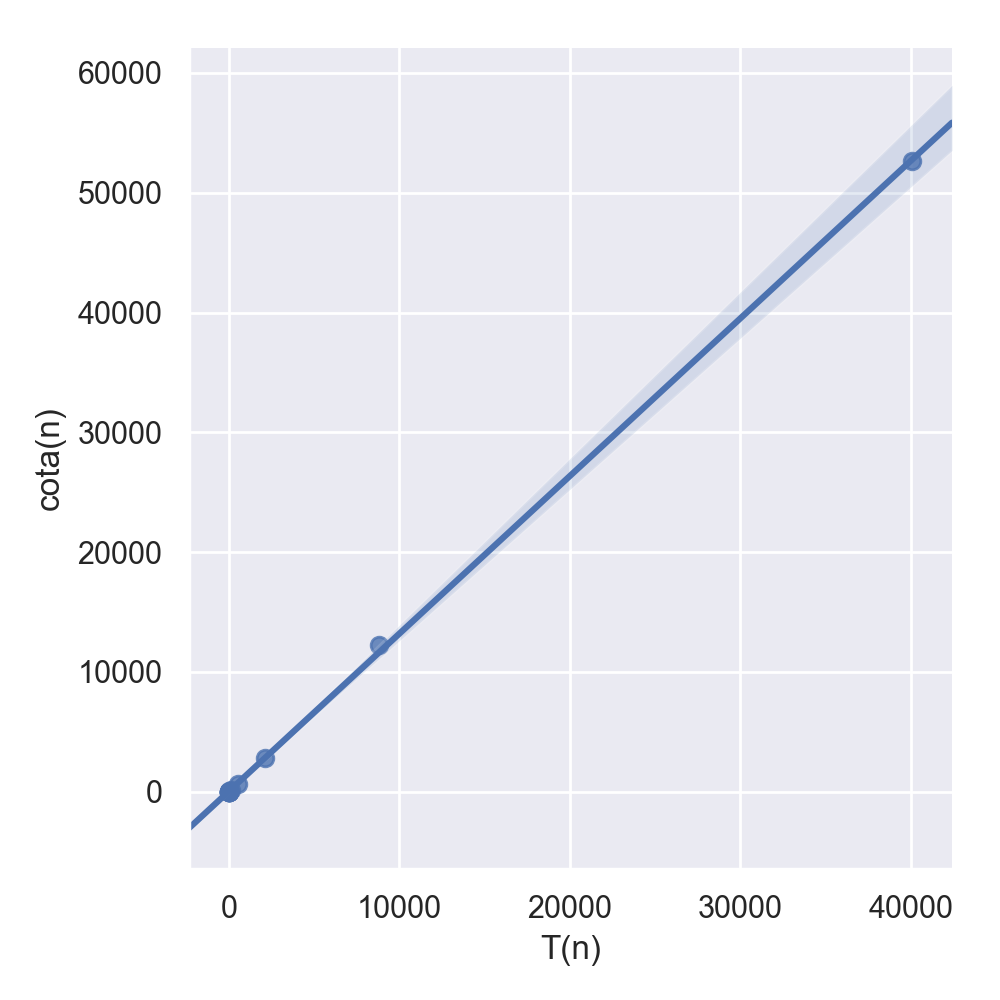
\includegraphics[width=1\linewidth]{img/fb_2}
     \caption{Correlación entre algoritmo y cota teórica}
   \end{minipage}
\end{figure}

En el primer gráfico podemos observar que la cota teórica se ajusta bien a el tiempo calculado y difiere mínimamente. Podemos considerar que esto se debe a constantes menores que puede tener el algoritmo con respecto a la cota superior calculada, pero sin embargo, esta diferencia también puede deberse a que no fue posible experimentar con valores grandes de N, dado que el tiempo de ejecución no nos lo permitió.
\newline
Ésta pequeña diferencia se la puede observar en el segundo gráfico. En este caso, podemos ver que nuestros datos tienen una correlación positiva con la cota. Cálculando el coeficiente de correlación de Pearson, obtenemos un resultado de 0.9999204732522591, lo que nos confirma que los datos tienen una relación positiva casi perfecta.

\subsection{Experimentación sobre el algoritmo de Meet in the Middle}

En el caso de Meet in the Middle, variamos N en un rango de 0 a 50, y comparamos nuestros resultados con la cota teórica O($n*2^{n/2}$). Los siguientes gráficos muestran nuestros resultados:

\begin{figure}[H]
   \begin{minipage}{0.5\textwidth}
     \centering
     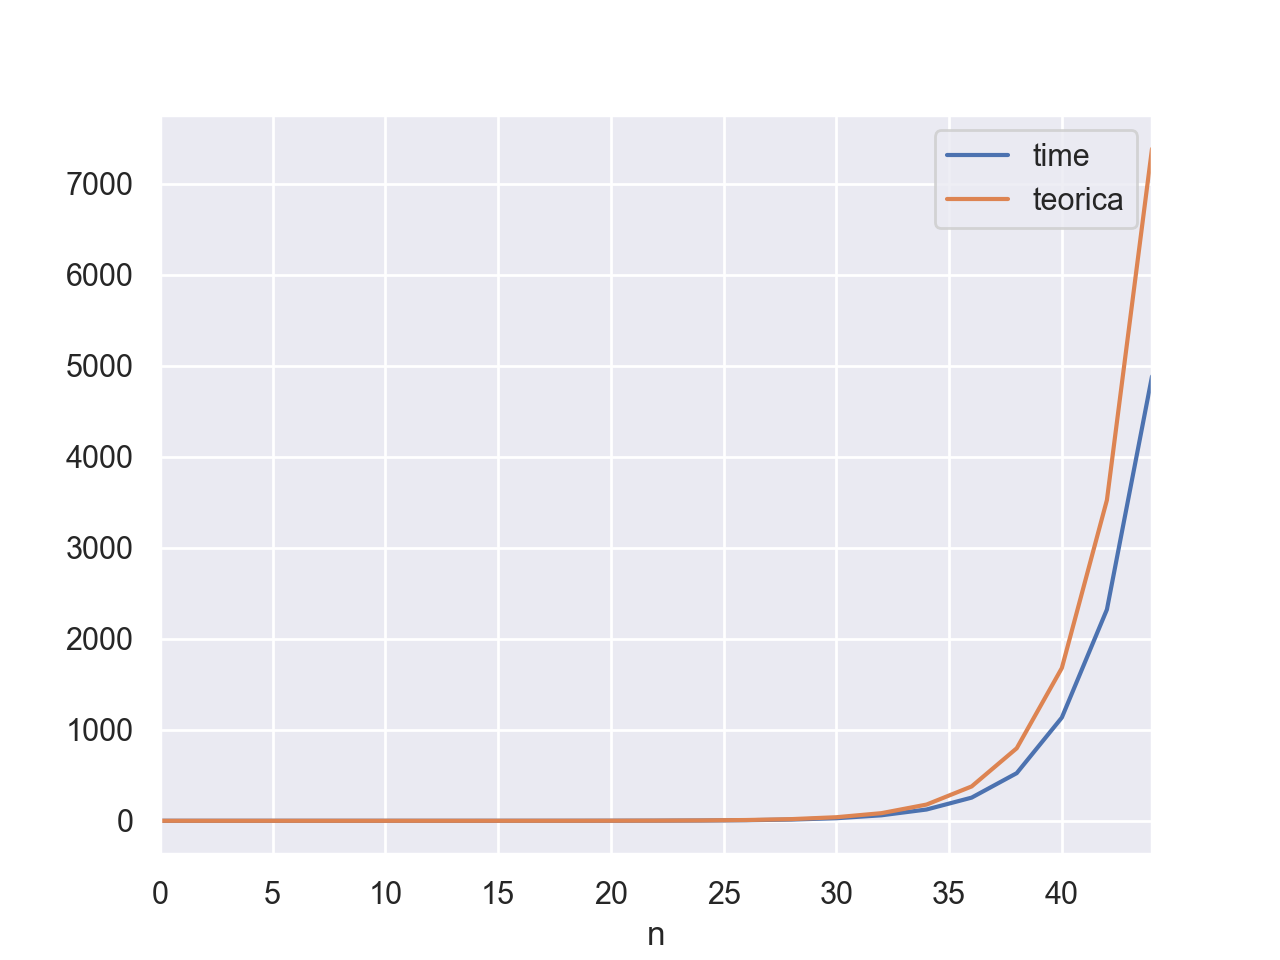
\includegraphics[width=1\linewidth]{img/Middle1}
     \caption{Comparación del gráfico de los resultados contra la cota teórica}
   \end{minipage}\hfill
   \begin{minipage}{0.5\textwidth}
     \centering
     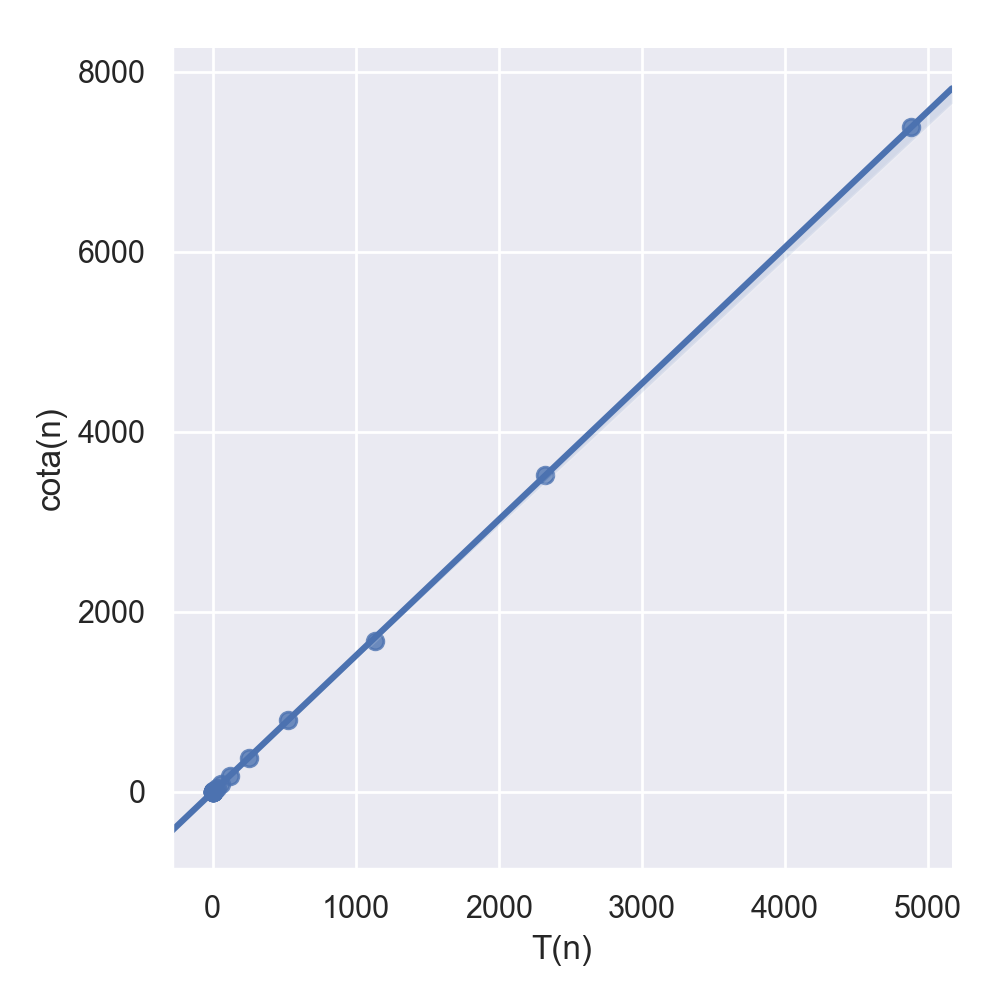
\includegraphics[width=1\linewidth]{img/Middle2}
     \caption{Correlación entre algoritmo y cota teórica}
   \end{minipage}
\end{figure}

Como podemos observar en el primer gráfico, parecería ser que el tiempo de ejecución se ajusta fuertemente a la cota teórica. Ambas funciones parecen tener un crecimiento similar, pero podemos corroborar esto más apropiadamente con el segundo gráfico. Aquí, vemos que nuestros datos tienen una correlación positiva casi perfecta con la cota teórica ya que la recta de cuadrados mínimos cubre casi perfectamente a nuestros datos. Para corroborar, calculamos el coeficiente de correlación de Pearson y obtuvimos un resultado de 0.9999865200267454, confirmando que nuestros datos tienen una relación positiva casi perfecta con la cota teórica.
\label{sec:experimentacion}



\subsection{Experimentación sobre el algoritmo de Backtracking}
Para el algoritmo de backtracking, comenzamos con un análisis del caso en el que no aplicamos ninguna poda. Como vimos en la sección anterior, tenemos una cota teórica de O($n*2^{n}$). Para ver que tan bien se ajusta nuestro algoritmo a ésta cota, generamos nuestros casos de test variando N entre 0 y 30. Veamos los resultados:

\begin{figure}[H]
   \begin{minipage}{0.5\textwidth}
     \centering
     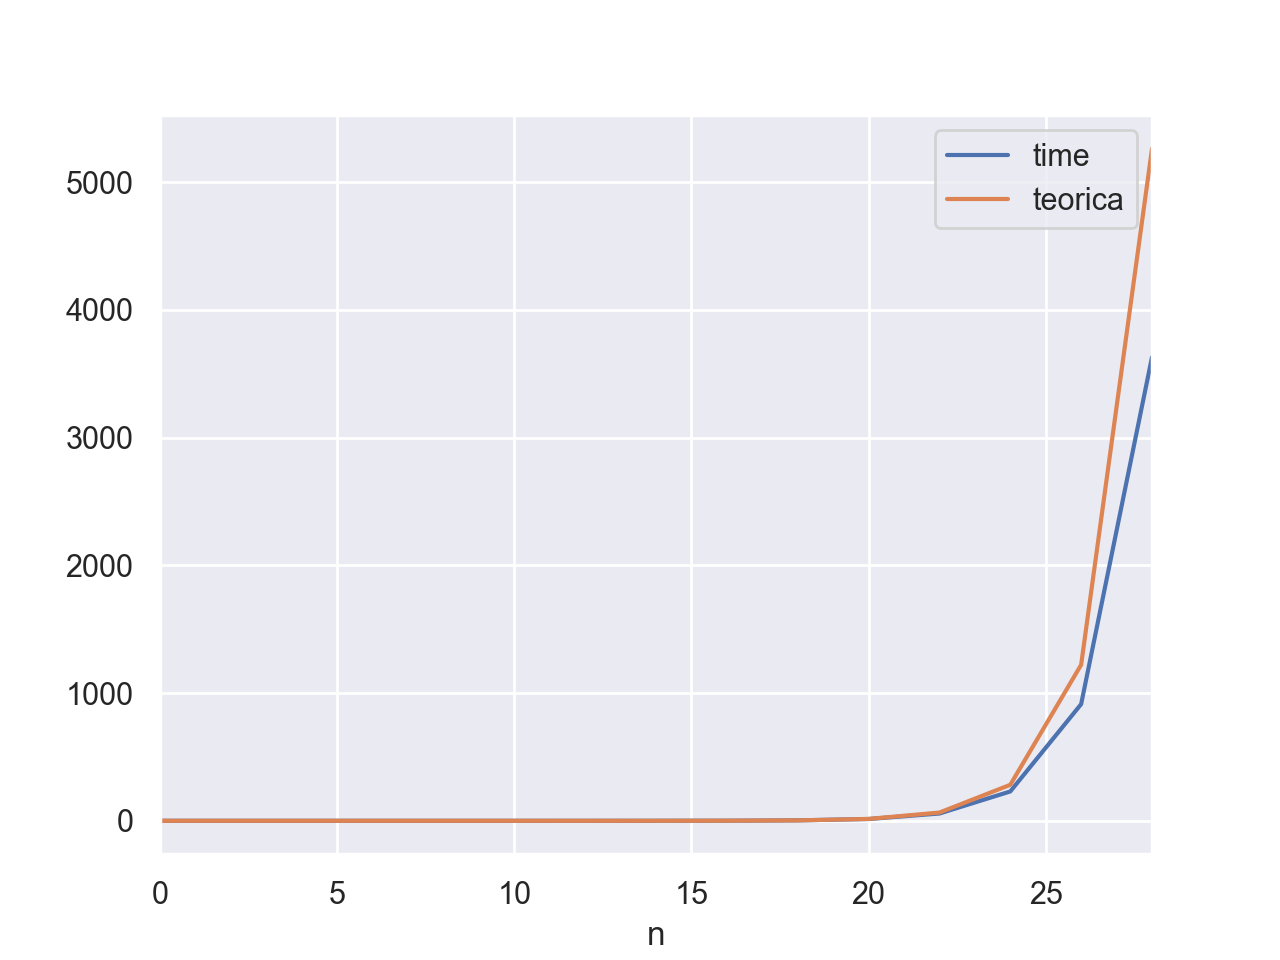
\includegraphics[width=1\linewidth]{img/sinPodas1}
     \caption{Comparación del gráfico de los resultados contra la cota teórica}
   \end{minipage}\hfill
   \begin{minipage}{0.5\textwidth}
     \centering
     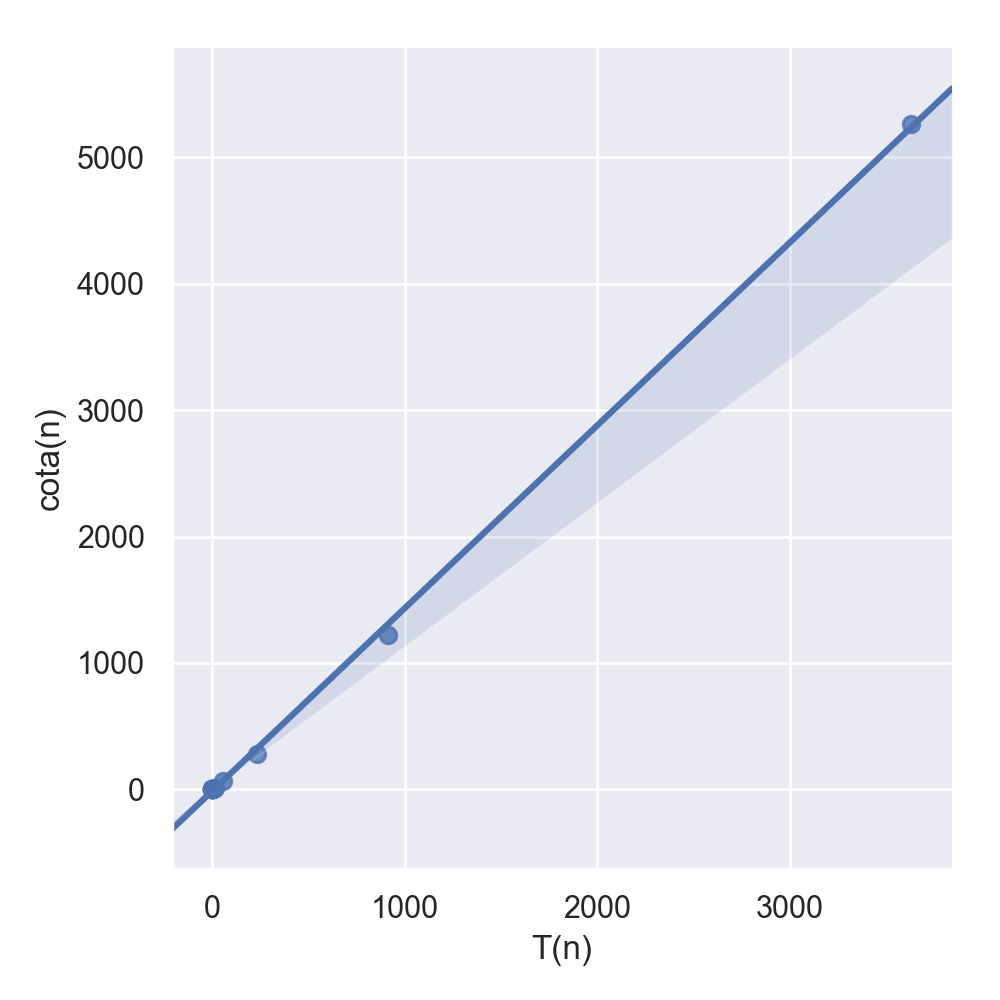
\includegraphics[width=1\linewidth]{img/sinPodas2}
     \caption{Correlación entre algoritmo y cota teórica}
   \end{minipage}
\end{figure}

Como podemos observar en el primer gráfico, la cota teórica tiene un crecimiento un poco más acelerado que nuestros datos. Esto es un resultado que nos sorprende, ya que como vimos antes, la complejidad de éste algoritmo se puede calcular de manera sencilla. Creemos que esta diferencia puede deberse a que no fue posible experimentar demasiados valores de N, dado que el tiempo de ejecución no nos lo permitió.
\newline
Ésta misma diferencia se ve plasmada en el segundo gráfico. En este caso, podemos ver que nuestros datos tienen una correlación positiva con la cota que, aunque es bastante fuerte, no es tan ajustada como por ejemplo en el algoritmo de Meet in the Middle. En particular, obtuvimos un coeficiente de correlación de Pearson de 0.9997870087191989, que parece indicar una correlación más fuerte que la que sugiere el gráfico.

\bigskip

Pasemos a ver que sucede cuando agregamos las podas. En este caso, quisimos comparar que sucedía tanto en el mejor caso como en el peor caso de una entrada dada. Es decir, dado un conjunto de elementos de entrada, las formas en la que más podamos y la que menos. Para lograr esto, variamos N en un rango de 0 a 50, y en cada caso ordenamos los elementos de distinta manera:
\begin{itemize}
\item Para lograr el mejor caso, ordenamos los elementos de mayor a menor respecto al peso y al beneficio. Este orden se debe a que, por un lado, podamos cuando nos pasamos del peso límite W. Por este motivo, poner los elementos más pesados al principio hace que podemos más rápidamente. Por otro lado, podamos cuando la suma de todos los beneficios que quedan no es suficiente para alcanzar a nuestra mejor solución hasta el momento. Así, tener los beneficios más bajos al final minimiza esta suma, logrando que podemos antes.
\item Para lograr el peor caso, usamos el orden opuesto, es decir, ordenamos de menor a mayor respecto al peso y al beneficio. Esto nos lleva al peor caso por los motivos opuestos a los recién mencionados.
\end{itemize}

Veamos como se comparan en un gráfico:


\begin{figure}[H]
     \centering
     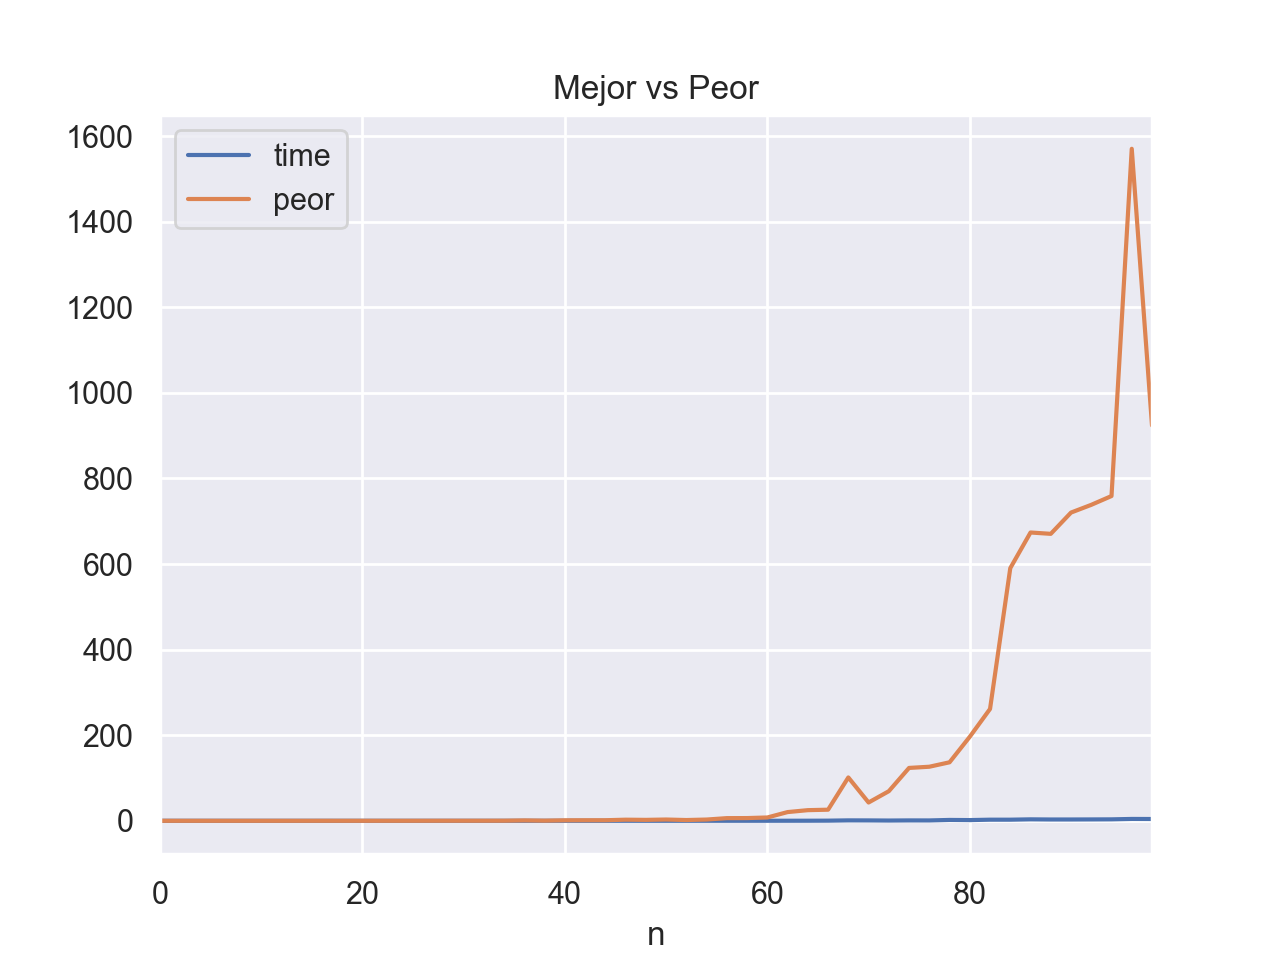
\includegraphics[width=0.7\linewidth]{img/mejor_peor_1}
     \caption{mejor vs peor caso}
\end{figure}

Para realizar este gráfico, corrimos ambos casos variando n entre 0 y 100. Como podemos observar, la diferencia entre ambos es abismal. Ésto nos habla de la importancia que tiene encontrar buenas podas para los algoritmos de backtracking, ya que en la práctica son las podas las que los diferencian de otros algoritmos de fuerza bruta. Para darnos una idea númerica, cuando N=5, el peor caso tarda 53 veces más que el mejor, y cuando N=96 tarda 363 veces más.

Por otro lado, queremos ver como se ajusta el algoritmo de backtracking con podas a nuestra cota teórica:

\begin{figure}[H]
   \begin{minipage}{0.5\textwidth}
     \centering
     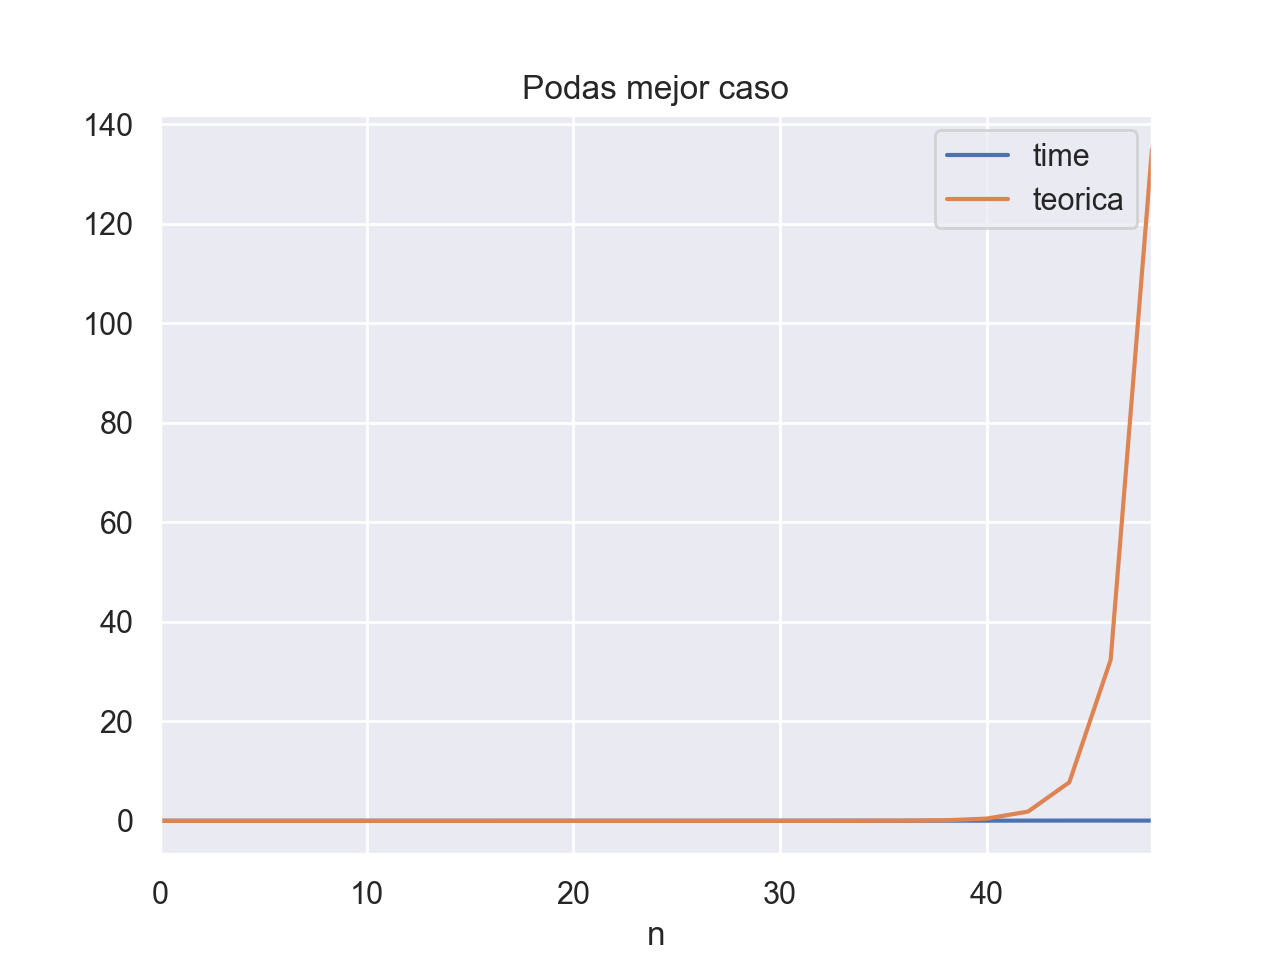
\includegraphics[width=1\linewidth]{img/mejor_Figure_1}
     \caption{Comparación del gráfico de los resultados contra la cota teórica}
   \end{minipage}\hfill
   \begin{minipage}{0.5\textwidth}
     \centering
     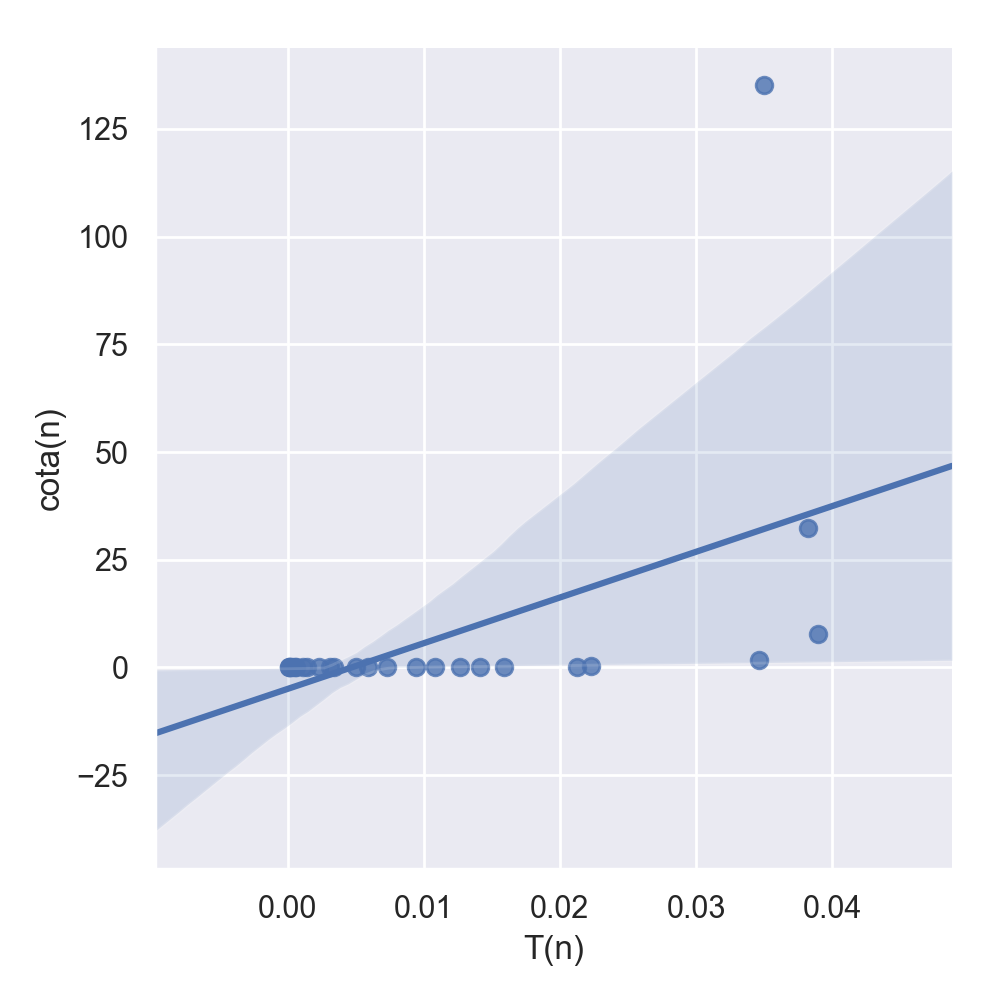
\includegraphics[width=1\linewidth]{img/mejor_Figure_2}
     \caption{Correlación entre algoritmo y cota teórica}
   \end{minipage}
\end{figure}

A partir de ambos gráficos podemos conjeturar que en el caso de backtracking con podas, no tenemos una buena correlación entre los datos y la cota teórica. En particular, el coeficiente de correlación de Pearson en este caso es de -0.09510266610231015, lo que parece indicar que prácticamente no hay correlación entre los datos y la cota teórica. Ésto se debe a que en todos nuestros casos aleatoriamente generados, el algoritmo logra podar una gran cantidad de ramas del árbol de backtracking. Sin embargo ésto no quiere decir que la cota no sea ajustada. Podríamos encontrar un cierto conjunto de datos de entrada que hagan que el algoritmo no haga ninguna poda, y en esos casos los resultados serían muy similares a los del análisis de backtracking sin podas. Por ejemplo, si la suma total de los pesos nunca sobrepasa al límite W, nunca realizaríamos nuestra poda por factibildad. Más aún, si el conjunto que contiene a todos los elementos es el último que revisamos, tampoco realizaríamos nuestra poda por optimalidad.


\subsection{Experimentación sobre el algoritmo de Programación Dinámica}
Para el algoritmo de Programación Dinámica notamos, al igual que en el algoritmo de fuerza bruta, que no importa el valor de la instancia pues siempre recorremos todo la matriz, por lo tanto si importa tanto el valor de N como de W. Como vimos en la sección anterior, tenemos una cota teórica de O($NxW$). Para ver que tan bien se ajusta nuestro algoritmo a ésta cota, experimentamos generando instancias aleatorias variando N y W, ambos entre 0 y 50. Veamos los resultados:
\begin{center}

\begin{figure}[H]
     \centering
     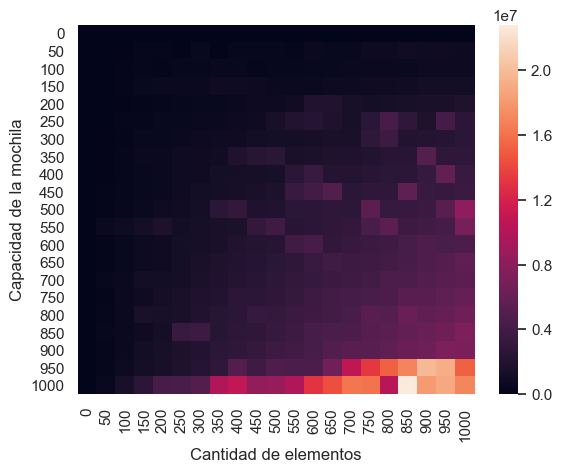
\includegraphics[width=0.5\linewidth]{img/heatmap}
     \caption{tiempos del algoritmo correspondiente a los valores de N y W}
\end{figure}

\end{center}
En el heatmap podemos observar como ambos valores (N y W) influyen en el tiempo de ejecución de nuestro algoritmo, ya que para valores grandes de ambos el algoritmo toma el mayor tiempo, y cuando alguno de los dos valores es chico el algoritmo toma poco tiempo.

A su vez, para poder verificar que nuestro algoritmo corre en tiempo lineal cuando una de las dos variables esta fija, realizamos el experimento de fijar una variable (en este caso $w=25$) y variar la otra variable ($n$) y ver el tiempo que toma el algoritmo. Veamos los resultados:

\begin{figure}[H]
   \begin{minipage}{0.5\textwidth}
     \centering
     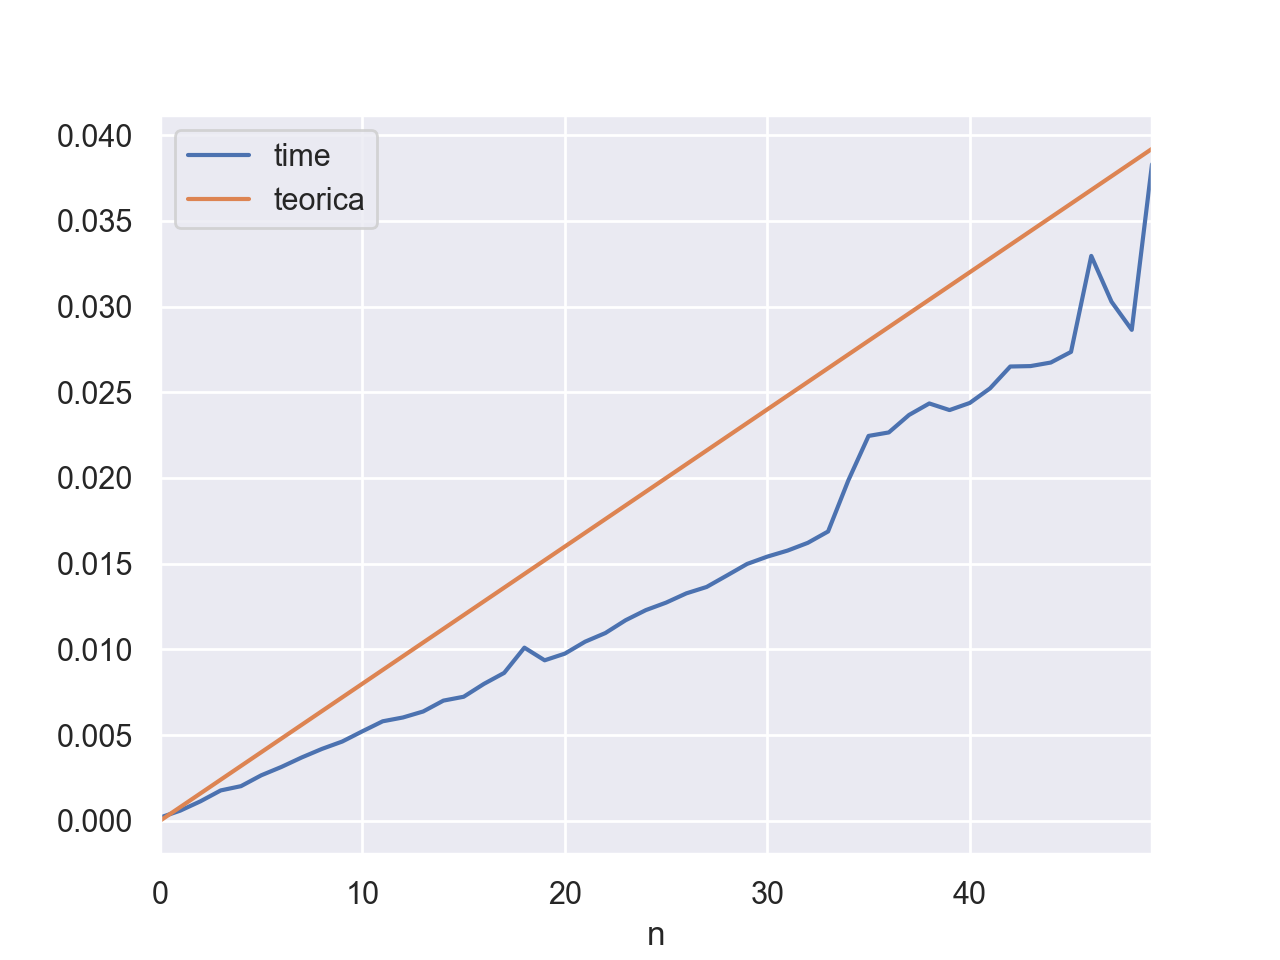
\includegraphics[width=1\linewidth]{img/fijo_w_1}
     \caption{Comparación del gráfico de los resultados contra la cota teórica con $w=25$}
   \end{minipage}\hfill
   \begin{minipage}{0.5\textwidth}
     \centering
     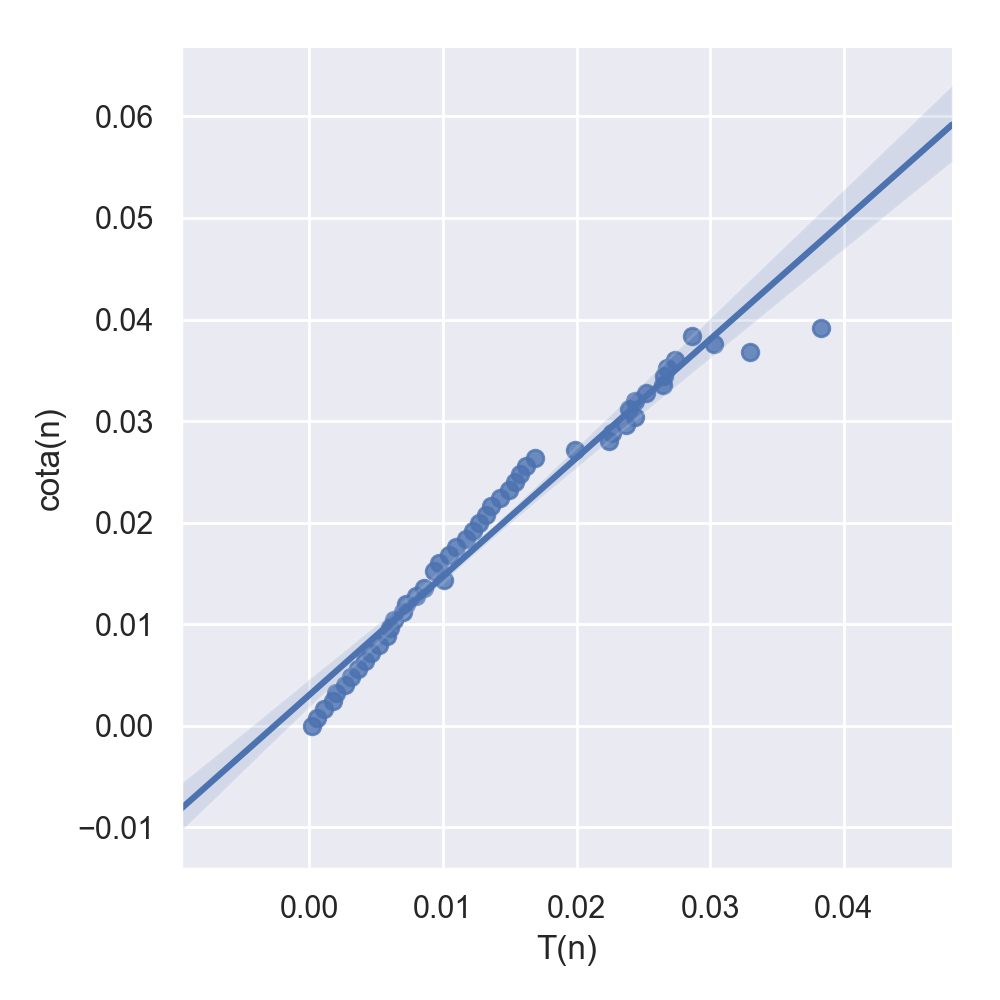
\includegraphics[width=1\linewidth]{img/fijo_w_2}
     \caption{Correlación entre algoritmo y cota teórica con $w=25$}
   \end{minipage}
\end{figure}


Como podemos observar en el primer gráfico, el tiempo de ejecución del algoritmo se encuentra acotado superiormente por una función lineal, lo cual verifica nuestra hipótesis inicial, ya que al fijar una variable el tiempo solo aumenta linealmente en función de la variable $N$. Para corroborar esto de nuevo, planteamos un segundo gráfico que muestra la correlación entre el algoritmo y la cota teórica propuesta. En este caso, podemos ver que nuestros datos tienen una correlación positiva con la cota que, aunque es bastante fuerte, no es tan ajustada como por ejemplo en el algoritmo de Meet in the Middle. Más específicamente, el coeficiente de correlación de Pearson en este caso fue de 0.9804304907022177 que, como vimos en el gráfico, es una correlación positiva fuerte, pero más débil que en la mayoría de los otros algorítmos calculados.

\subsection*{Comparacion entre Fuerza Bruta y backtracking sin podas}
Tanto el algoritmo de Fuerza Bruta como el de Backtracking sin podas tienen la misma complejidad, O($n*2^{n}$). Veamos como se comparan empíricamente:

\begin{figure}[H]
   \begin{minipage}{0.5\textwidth}
     \centering
     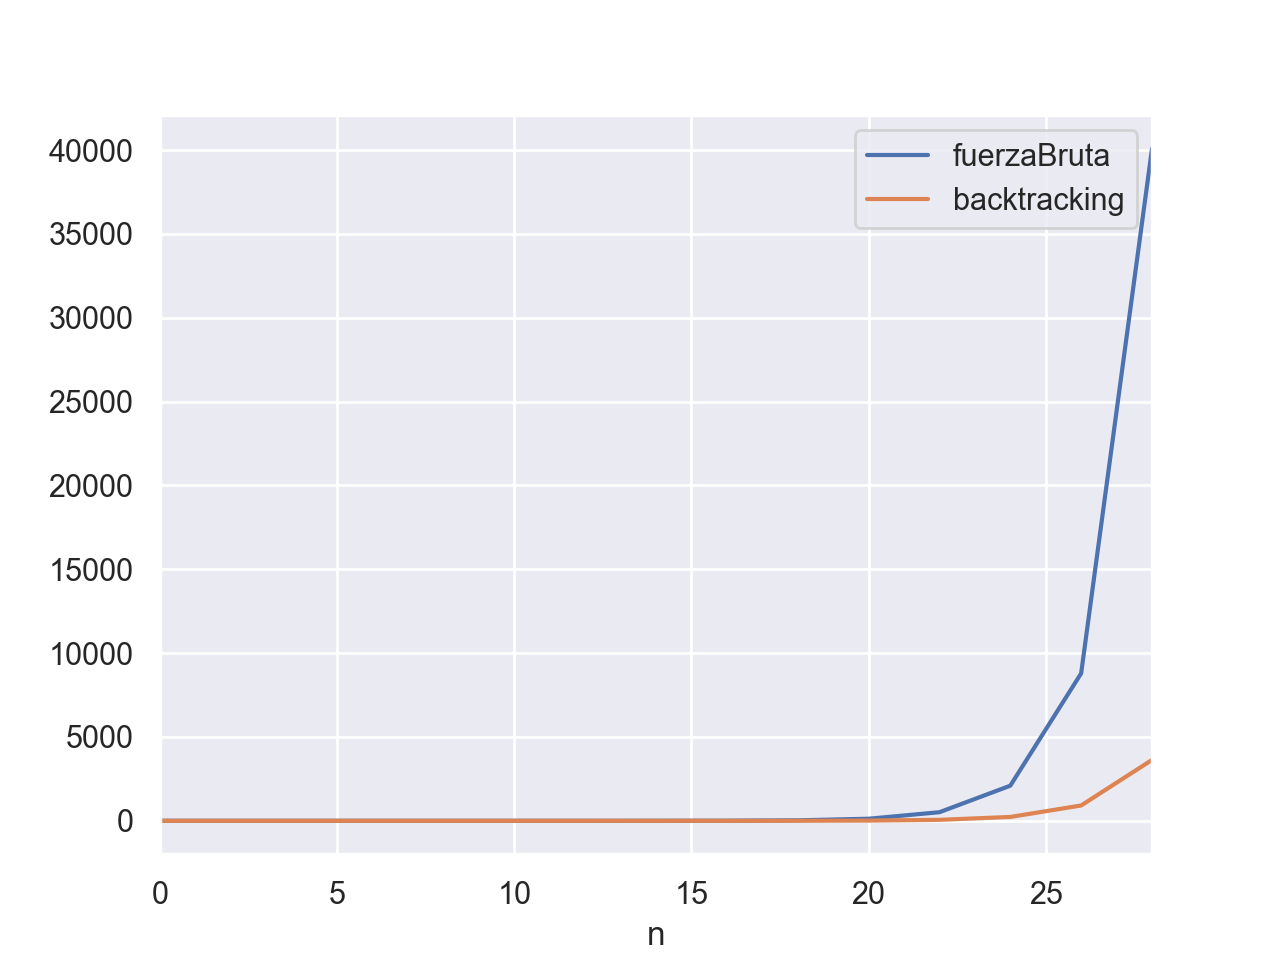
\includegraphics[width=1\linewidth]{img/fb_vs_bt_1}
     \caption{Comparación entre la complejidad de los algoritmos}
   \end{minipage}\hfill
   \begin{minipage}{0.5\textwidth}
     \centering
     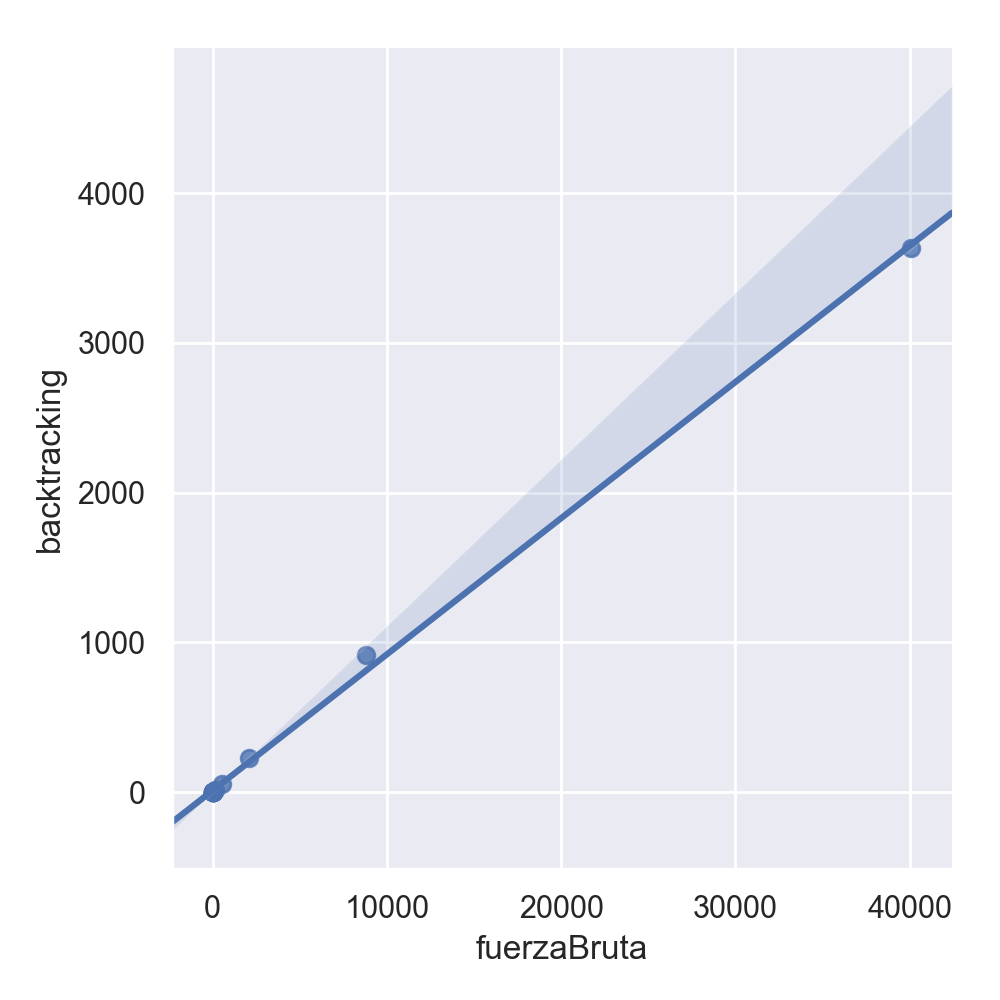
\includegraphics[width=1\linewidth]{img/fb_vs_bt_2}
     \caption{Correlación entre las complejidades de los algoritmos}
   \end{minipage}
\end{figure}

Como podemos ver, el algoritmo de Backtracking parece ser más rápido que el de Fuerza Bruta, aunque presentan una correlación positiva bastante fuerte.

\subsection*{Comparacion entre Fuerza Bruta y Meet in the Middle}
Comparemos ahora el algoritmo de Fuerza Bruta con uno de  mejor complejidad, Meet in the Middle:

\begin{figure}[H]
   \begin{minipage}{0.5\textwidth}
     \centering
     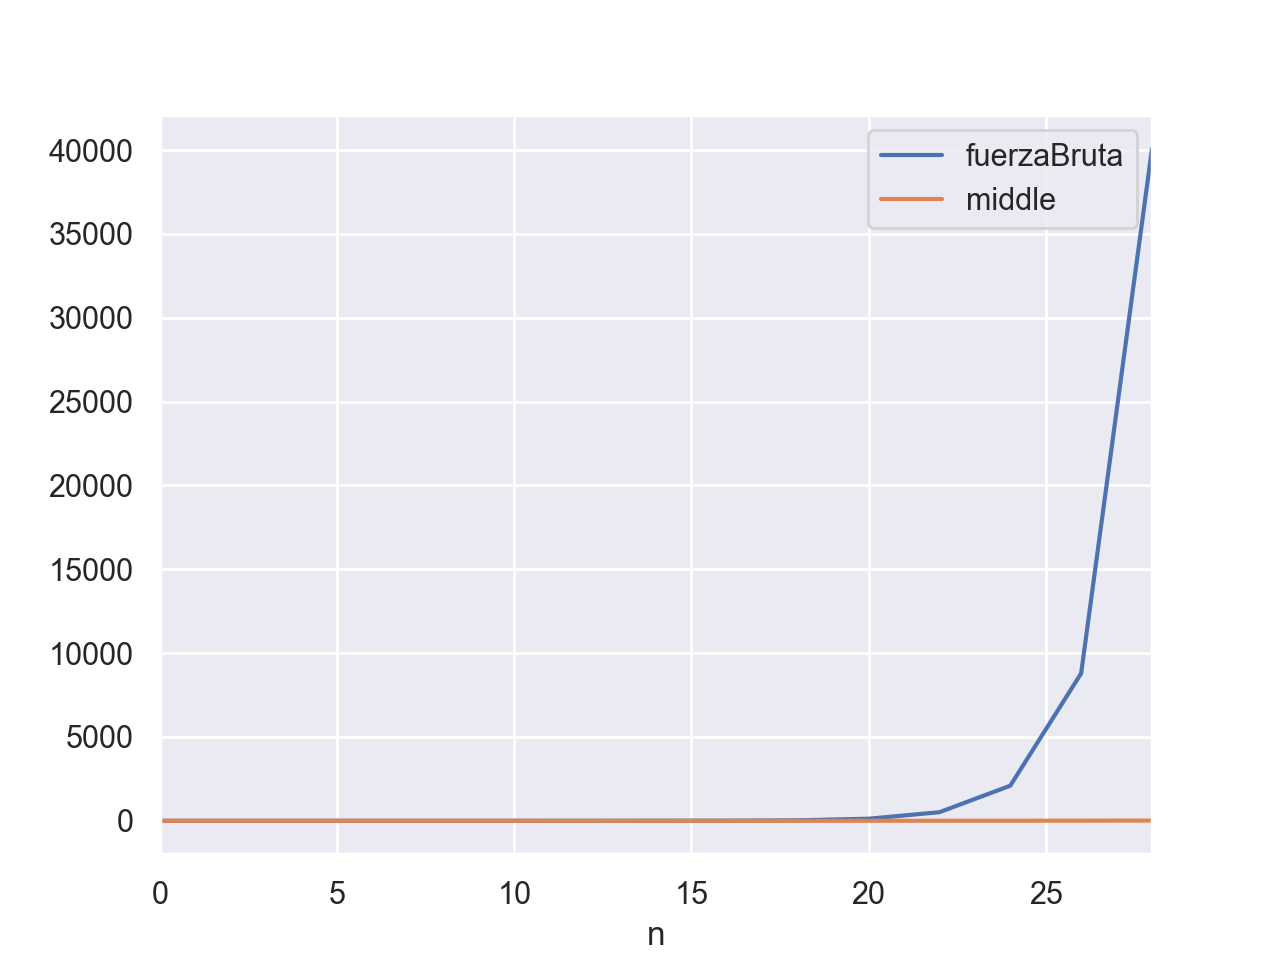
\includegraphics[width=1\linewidth]{img/fb_vs_middle_1}
     \caption{Comparación entre la complejidad de los algoritmos}
   \end{minipage}\hfill
   \begin{minipage}{0.5\textwidth}
     \centering
     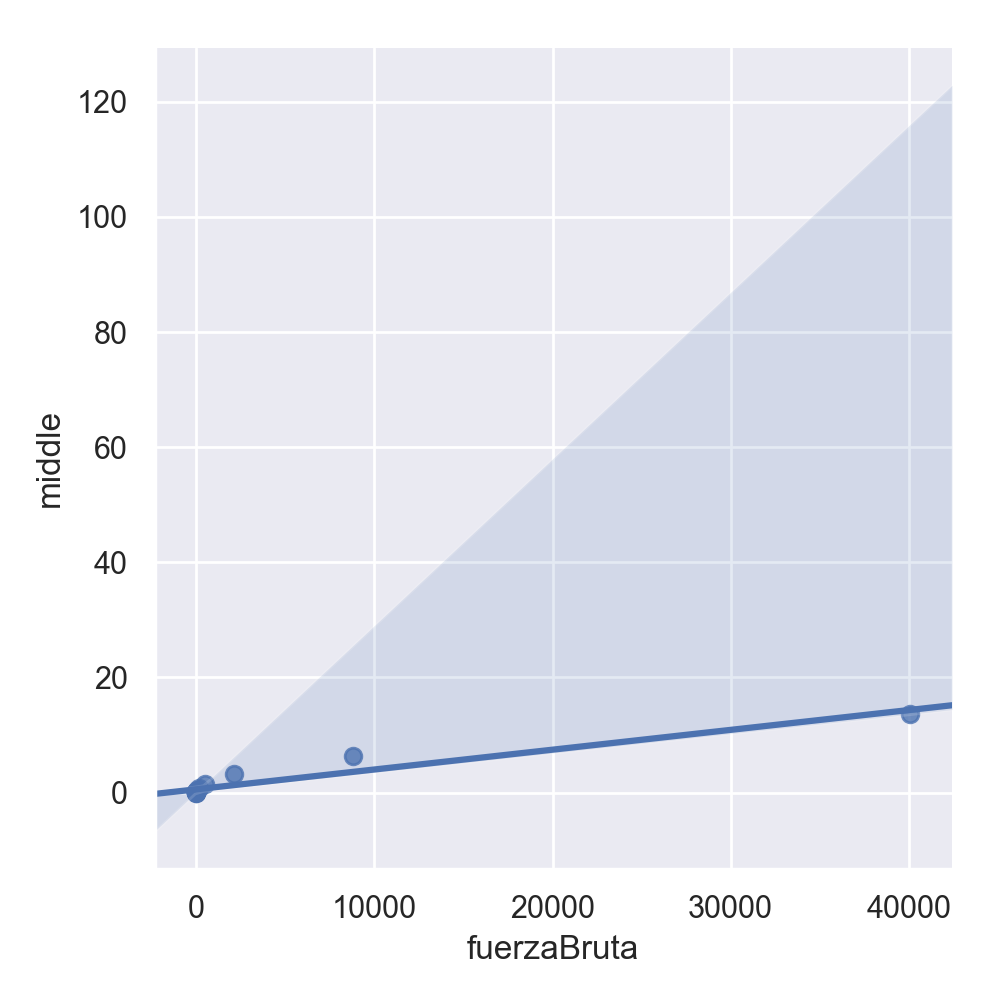
\includegraphics[width=1\linewidth]{img/fb_vs_middle_2}
     \caption{Correlación entre las complejidades de los algoritmos}
   \end{minipage}
\end{figure}

En este caso, vemos como el algoritmo de Meet in the Middle es mucho más rápido que el de Fuerza Bruta. En el segundo gráfico, vemos como la recta de cuadrados mínimos tiene una pendiente muy pequeña, lo que nos estaría mostrando como el algoritmo de Fuerza Bruta crece tanto más rápido que el de Meet in the Middle.
